\documentclass{article}
\usepackage{tikz}
\usetikzlibrary{shapes.geometric, arrows}

\tikzstyle{startstop} = [rectangle, rounded corners, minimum width=3cm, minimum height=1cm,text centered, draw=black, fill=red!30]
\tikzstyle{process} = [rectangle, minimum width=3cm, minimum height=1cm, text centered, draw=black, fill=blue!30]
\tikzstyle{decision} = [diamond, minimum width=3cm, minimum height=1cm, text centered, draw=black, fill=green!30]
\tikzstyle{arrow} = [thick,->,>=stealth]

\begin{document}

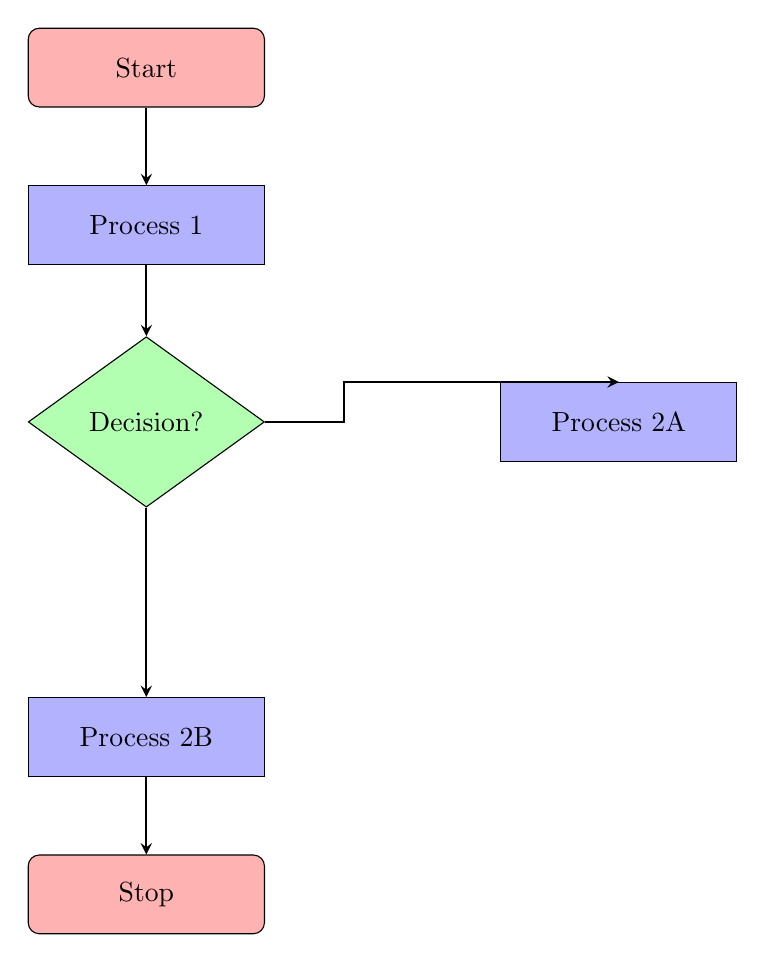
\begin{tikzpicture}[node distance=2cm]

% Nodes
\node (start) [startstop] {Start};
\node (process1) [process, below of=start] {Process 1};
\node (decision1) [decision, below of=process1, yshift=-0.5cm] {Decision?};
\node (process2a) [process, right of=decision1, xshift=4cm] {Process 2A};
\node (process2b) [process, below of=decision1, yshift=-2cm] {Process 2B};
\node (stop) [startstop, below of=process2b] {Stop};

% Arrows
\draw [arrow] (start) -- (process1);
\draw [arrow] (process1) -- (decision1);
\draw [arrow] (decision1.east) -- ++(1,0) |- (process2a.north);
\draw [arrow] (decision1.south) -- (process2b.north);
\draw [arrow] (process2b) -- (stop);

\end{tikzpicture}

\end{document}
